\section{Allocazione di Memoria al Kernel}
Il kernel utilizza della memoria separata da quella destinata agli utenti, questa memoria molto spesso non è soggetta a paginazione in quanto esso opera con oggetti di piccole dimensioni che sprecherebbero le pagine.

Inoltre alcune parti della memoria del kernel devono essere contigue per permettere a dispositivi I/O, che non hanno accesso alla memoria fisica, di scriverci.

\spacer
Vedremo ora due tecniche per gestire la memoria che viene riservata al kernel.

\subsection{Allocatore potenza 2}
Utilizza un segmento di memoria a dimensione fissa e fisicamente contigua, che viene allocato in blocchi di dimensione pari a potenze del 2.

\spacer
Quando viene richiesta una quantità di memoria essa viene arrotondata alla più piccola potenza che la contiene, se si richiede una quantità di memoria minore il segmento viene diviso a metà.

\begin{figure}[H]
    \centering
    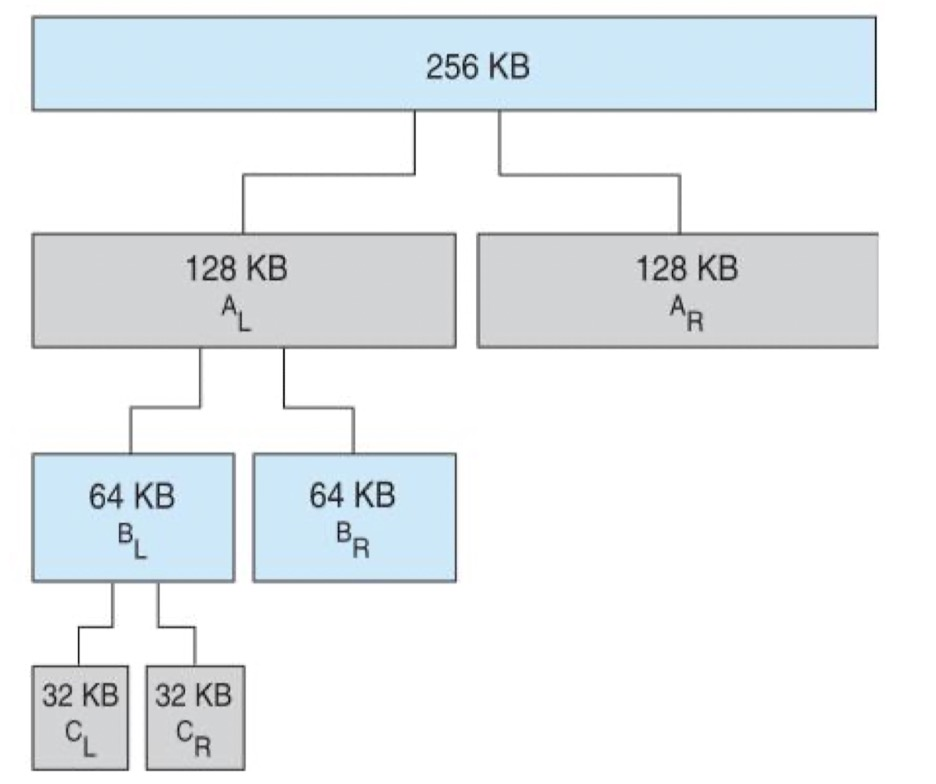
\includegraphics[width=0.4\linewidth]{assets/allocatore-potenza-2.jpg}
\end{figure}

\subsection{Allocazione a Lastra}
Il kernel ha la necessità di allocare e distruggere oggetti frequentemente, per questo motivo è conveniente mantenere una cache per ogni tipo di oggetto così da rimuovere il costo di inizializzazione.

\spacer
Le cache contengono istanze della struttura dati del kernel a cui sono assegnate e vengono inserite in una lastra (\textit{slab}), dei segmenti di memoria fisicamente contigui.

\spacer
Quando il kernel richiede un nuovo oggetto esso viene preso da quelli segnati come liberi.

Se non dovessero essere disponibili oggetti liberi ne vengono allocati altri in una lastra vuota. Nel caso in cui non dovessero esserci lastre libere verrà allocato spazio per far crescere la cache di una lastra.

\begin{figure}[H]
    \centering
    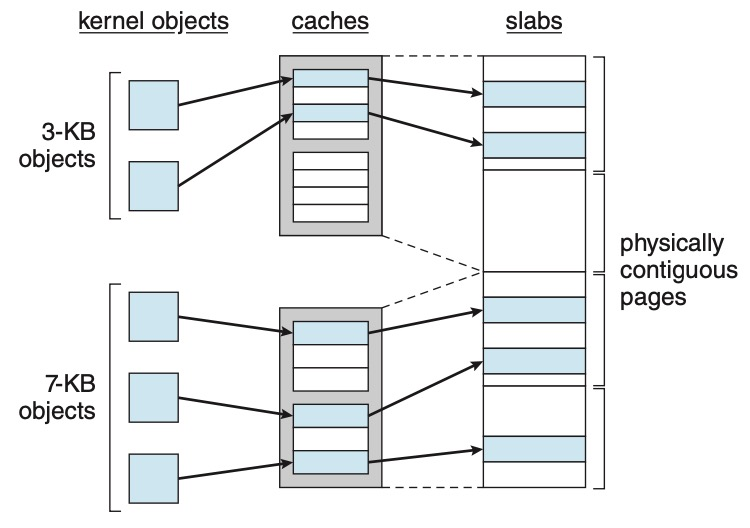
\includegraphics[width=0.5\linewidth]{assets/allocatore-lastra.jpg}
\end{figure}
